\documentclass[10pt]{article}

\usepackage[T1]{fontenc}
\usepackage[left=2cm, right=2cm, top=2cm, bottom=2cm]{geometry}
\usepackage[skins]{tcolorbox}
\usepackage{hyperref, fancyhdr, lastpage, tocloft, ragged2e, multicol}
\usepackage{amsmath, amssymb, amsthm}
\usepackage{tkz-tab}

\def\pagetitle{Fonctions usuelles}

\title{\bf{\pagetitle}\\\large{Corrigé}}
\date{Septembre 2023}
\author{DARVOUX Théo}

\DeclareMathOperator{\ch}{ch}
\DeclareMathOperator{\sh}{sh}
\DeclareMathOperator{\tah}{th}

\hypersetup{
    colorlinks=true,
    citecolor=black,
    linktoc=all,
    linkcolor=blue
}

\pagestyle{fancy}
\cfoot{\thepage\ sur \pageref*{LastPage}}


\begin{document}
\renewcommand*\contentsname{Exercices.}
\renewcommand*{\cftsecleader}{\cftdotfill{\cftdotsep}}
\maketitle
\hrule
\tableofcontents
\vspace{0.5cm}
\hrule

\thispagestyle{fancy}
\fancyhead[L]{MP2I Paul Valéry}
\fancyhead[C]{\pagetitle}
\fancyhead[R]{2023-2024}
\allowdisplaybreaks

\pagebreak
\addcontentsline{toc}{section}{Vocabulaire sur les fonctions.}

\section*{Exercice 4.1 [$\blacklozenge\lozenge\lozenge$]}
\begin{tcolorbox}[enhanced, width=7in, center, size=fbox, fontupper=\large, drop shadow southwest]
    Soit $f:\mathbb{R}\rightarrow\mathbb{R}$ une fonction $2$-périodique et $3$-périodique. Montrer que $f$ est $1$-périodique.\\
    On a :
    \begin{align*}
        \forall{x\in\mathbb{R}}\begin{cases}x-2\in\mathbb{R}\\f(x-2)=f(x)\end{cases} \text{ et } \begin{cases}x+3\in\mathbb{R}\\f(x+3)=f(x)\end{cases}
    \end{align*}
    Alors :
    \begin{align*}
        \forall{x\in\mathbb{R}}\begin{cases}x-2+3\in\mathbb{R}\\f(x-2+3)=f(x-2)=f(x)\end{cases}
    \end{align*}
    \qed
\end{tcolorbox}
\addcontentsline{toc}{section}{\protect\numberline{}Exercice 4.1}

\section*{Exercice 4.2 [$\blacklozenge\blacklozenge\blacklozenge$]}
\begin{tcolorbox}[enhanced, width=7in, center, size=fbox, fontupper=\large, drop shadow southwest]
    Déterminer toutes les fonctions croissantes $f:\mathbb{R}\rightarrow\mathbb{R}$ telles que
    \begin{equation*}
        \forall{x\in\mathbb{R}} \hspace{0.25cm} f(f(x))=x.
    \end{equation*}
    Soit $x\in\mathbb{R}$ et $f$ une solution du problème.\\
    On remarque que $f:x\mapsto x$ est solution du problème.\\
    Supposons $f(x)>x$, on a : $f(f(x))>f(x)$ par croissance de $f$. Or $f(f(x))=x$ donc $x>f(x)$, ce qui est absurde.\\
    Supposons $f(x)<x$, on a : $f(f(x))<f(x)$ par croissance de $f$. Or $f(f(x))=x$ donc $x<f(x)$, ce qui est absurde.\\
    Ainsi, la seule fonction de $\mathbb{R}$ vers $\mathbb{R}$ solution est $f:x\mapsto x$.
\end{tcolorbox}
\addcontentsline{toc}{section}{\protect\numberline{}Exercice 4.2}

\addcontentsline{toc}{section}{Étude de fonctions.}
\section*{Exercice 4.3 [$\blacklozenge\lozenge\lozenge$] S'entraîner tout seul à dériver.}
\begin{tcolorbox}[enhanced, width=7in, center, size=fbox, fontupper=\large, drop shadow southwest]
    Pour chacune des fonctions ci-dessous, donner un ou plusieurs intervalles sur lesquels la fonction est dérivable, et préciser sa dérivée.
    \begin{center}
        $A:x\mapsto x^\pi,\hspace{0.5cm}B:x\mapsto\pi^x,\hspace{0.5cm}C:x\mapsto\cos(5x),\hspace{0.5cm}D:x\mapsto\tah(\ch(x))$,\\
        $E:x\mapsto\ln\left(1+x^3\right)n\hspace{0.5cm}F:x\mapsto\cos\left(\sqrt{\ln(x)}\right),\hspace{0.5cm}G:x\mapsto\frac{1}{\sqrt{3x-1}},\hspace{0.5cm}H:x\mapsto\sin|x+1|$.
    \end{center}
    
    $G':x\mapsto-\frac{3}{2}(3x-1)^{3/2}$
    
    \begin{itemize}
        \item $A':\begin{cases}\mathbb{R}^*_+\rightarrow\mathbb{R}\\x\mapsto\pi x^{\pi-1}\end{cases}$\hspace{1.8cm}• $D':\begin{cases}\mathbb{R}\rightarrow\mathbb{R}\\x\mapsto\frac{\sh(x)}{\ch^2(\ch(x))}\end{cases}$\hspace{1.6cm}• $H'_-:\begin{cases}]-\infty,-1[\rightarrow\mathbb{R}\\x\mapsto-\cos(-x-1)\end{cases}$
        \item $B':\begin{cases}\mathbb{R}\rightarrow\mathbb{R}\\x\mapsto\ln(\pi)\pi^x\end{cases}$\hspace{1.5cm}• $E':\begin{cases}\mathbb{R}\setminus\{1\}\rightarrow\mathbb{R}\\x\mapsto\frac{3x^2}{1+x^3}\end{cases}$\hspace{1.6cm}• $H'_+:\begin{cases}]1,+\infty[\rightarrow\mathbb{R}\\x\mapsto\cos(x+1)\end{cases}$
        \item $C':\begin{cases}\mathbb{R}\rightarrow\mathbb{R}\\x\mapsto-5\sin(5x)\end{cases}$\hspace{1.0cm}• $F':\begin{cases}]1,+\infty[\rightarrow\mathbb{R}\\x\mapsto\frac{\sin(\sqrt{\ln(x)})}{2x\sqrt{\ln(x)}}\end{cases}$
    \end{itemize}
\end{tcolorbox}
\addcontentsline{toc}{section}{\protect\numberline{}Exercice 4.3}

\section*{Exercice 4.4 [$\blacklozenge\lozenge\lozenge$]}
\begin{tcolorbox}[enhanced, width=7in, center, size=fbox, fontupper=\large, drop shadow southwest]
    Donner le tableau de variations complet de
    \begin{equation*}
        f:x\mapsto x^{x\ln(x)}.
    \end{equation*}
    On a :
    \begin{equation*}
        f:x\mapsto e^{x\ln^2(x)}
    \end{equation*}
    Donc :
    \begin{equation*}
        f':\begin{cases}\mathbb{R}_+^*\rightarrow\mathbb{R}\\x\mapsto\ln(x)(\ln(x)+2)e^{x\ln^2(x)}\end{cases}
    \end{equation*}
    Son tableau de variations est donc :
    \begin{center}
        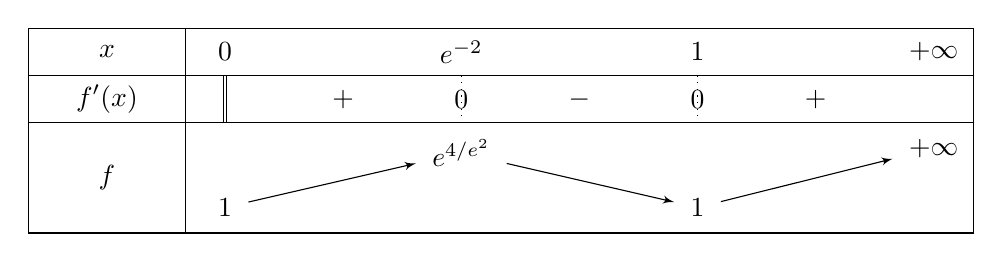
\begin{tikzpicture}
            \tkzTabInit[espcl=3]{$x$/0.6,$f'(x)$/0.6,$f$/1.4}{$0$,$e^{-2}$,$1$,$+\infty$}
            \tkzTabLine{d,+,z,-,z,+}
            \tkzTabVar{-/$1$,+/$e^{4/e^{2}}$,-/$1$,+/$+\infty$}
        \end{tikzpicture}
    \end{center}
\end{tcolorbox}
\addcontentsline{toc}{section}{\protect\numberline{}Exercice 4.4}

\end{document}